\subsection{Introduction}
The term "brain (or neural) oscillations" refers to the rhythmic and/or repetitive electrical 
activity generated spontaneously and in response to stimuli by neural tissue in the central 
nervous system. The importance of brain oscillations in sensory-cognitive processes has become 
increasingly evident. This chapter will focus on some questions:
\begin{itemize}
    \item What does a neural oscillation consist of and how does it originate?
    \item What are the (main) roles of brain oscillations?
    \item How dowe observe and characterize a brain oscillation?
\end{itemize}

\subsection{Neuronal Geometry and Architecture}
By looking at the extracellular field potentials, brain signals are strongly dependent on the 
geometry of the system (e.g., the hippocampus has a very different geometry with respect to 
the subthalamic nuclei). Based on the geometry and the architecture of the system, the signals 
could be very different.
\begin{itemize}
    \item Much of the signals taken into account are coming from \textbf{pyramidal cells}, because they have a very 
    specific geometry and orientation that create aligned electrical dipoles, which generate very strong 
    electrical field potentials.
    \item There are also \textbf{spherically symmetric neurons} (e.g., thalamocortical cells) which have a circular 
    geometry with dendrites of relatively equal size in all directions that somehow reduces the possibility of 
    having very synchronized field potentials.
\end{itemize}

\subsection{EEG and MEG}
Electroencephalography (EEG) and Magnetoencephalography (MEG) are the main classical techniques for recording 
non-invasively the electrical activity from the human brain. These two techniques can be combined with systems 
that record both the electrical field and the magnetic field, but, in general, they record two different aspects 
of the same event: there is a current that travels along the axons of the dendrites generating an electrical 
field that is summed among many cells and finally reaches the sensors. Depending on the physical variable that is 
taken into account, an EEG or a MEG can be recorded.
\begin{itemize}
    \item The EEG records the electrical field and, for this reason, the unit of measurement is volts (typically 
    microvolts, \(10^{-6} V\)).
    \item The MEG records the magnetic inducted component in a static magnetic field where the head of the person is 
    immersed on. The unit of measurement is tesla (typically femtotesla, which is \(10^{-15} T\)).
\end{itemize}
One of the major difference is the fact that the two systems are very different in terms of acquisition systems: EEG 
is composed by sensors placed on the scalp and wires (one for each electrode) connected to an amplifier, because 
electrical fields have a power that needs to be amplified, while MEG requires dedicated and specially built rooms and more 
intensive and expensive maintenance.
One drawback of the MEG is the fact that the coils are fixed, and so, if the subject moves his head, there is a 
a magnetic induction even though the current is not travelling, and data are completely useless.\\
One of the main reason for acquiring and looking at MEG instead of EEG is the fact that magnetic fields pass through the 
skull and scalp, whereas the electrical fields are volume conducted through these tissues, which decreases signal-to-noise 
ratio at higher frequencies (performing a low-pass filtering). For this reason, MEG signals have a larger power in terms of 
spatial resolution (better localization power), and this could be useful, for instance, for clinical purpose, as for studying 
epilepsy.

\subsection{Origin of EEG Signal}
This technique is not so different from what has been said regarding local field potentials, but it has one more problem: the sensors 
are not located into the brain but outside, and so the signal has to travel all the distance from the source up to the electrodes.
EEG is the synchronized synaptic activity in populations of cortical neurons closer to the electrode, performing a spatial integration 
(net sum at the electrode).
What is the problem of the spatial integration? There is a difference governed by the orientation of the neurons.
\par\medskip
Electrodes detect the sum of positive and negative charges in their vicinity. In the case where an electrode is equidistant from
both source (region of positive charge) and sink (region of negative charge) of a dipole, the electrode will measure a net
neutral; so, an electrode can only detect dipoles when the electrode is closer to either the positive or negative end of the dipole. 
This means that two major types of dipoles are measurable in EEG: tangential dipoles, which are oriented perpendicular to
the surface (first figure), and radial dipoles, which are oriented parallel to the scalp surface (second figure). Dipoles have a 
positive and negative side, and therefore will produce both a positive deflection and a negative deflection at different regions of the scalp.
\begin{figure}[H]
    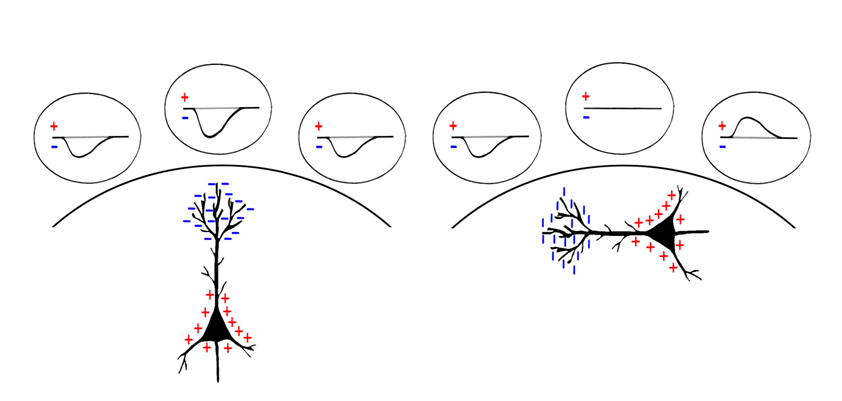
\includegraphics[scale=0.55]{10_1}
    \centering
\end{figure}
A single neuron's dipole is too small to be measured as far away as the scalp. However, because electrodes detect the sum of charges
in their vicinity, the dipoles from multiple neurons in a region will sum together. The sum of many individual dipoles in an area is
measurable as a single dipole whose magnitude reflects the number of neurons whose dipoles are summing together. However, because electrodes 
will measure the sum of both the positive and the negative ends of dipoles in the brain, in order to produce a measurable (nonzero) signal, 
neurons must be both arranged in a \textit{parallel manner}, and \textit{synchronously active}. The parallel arrangement is necessary to produce a measurable 
dipole because, if the neurons are all arrayed in the same orientation, then their signals can sum to form a larger signal. 
In any other configuration, the individual dipoles' positive and negative ends will sum and cancel each other out. The synchronization 
of activity is necessary in order to yield a net charge on the scalp-facing side of the dipole sheet, rather than charges cancelling each other out; 
and a signal large enough to be measured.

